\documentclass[tikz]{standalone}

\usepackage{tikz}
\usetikzlibrary{automata}

\begin{document}

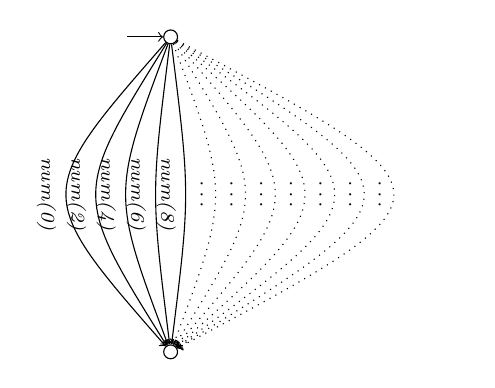
\begin{tikzpicture}
    \tikzstyle{every state}=[
        draw,
        shape=circle,
        inner sep=1pt,
        minimum size=5pt,
        final/.style={double,minimum size=6pt},
        initial text=]

    [auto,->]
    \renewcommand{\a}[1]{\textit{#1}}
    \node[state,initial] (n)  {};
    \node[state] (e) [below of=n, node distance=4cm] {};
    \foreach \n/\l in {0/0,1/2,2/4,3/6,4/8}
    \foreach \x in {-1.75cm+\n*0.5cm}
    \path[draw,->] (n) .. controls (\x,-2cm)..  (e) 
        node[sloped,below,pos=0.5]{\scriptsize\a{num(\l)}};
    \foreach \n in {5,...,11}
    \foreach \x in {-1.75cm+\n*0.5cm}
    \path[draw,->,dotted] (n) .. controls (\x,-2cm)..  (e) 
        node[sloped,below,pos=0.5]{\scriptsize$\cdots$};
\end{tikzpicture}
\end{document}